\documentclass[a4paper,11pt]{article}

\usepackage[french]{babel}
\usepackage[T1]{fontenc}
\usepackage[utf8]{inputenc}
\usepackage{graphicx}
%\usepackage{fullpage}

\begin{document}

\title{Compte rendu du TP \no 6\\\textbf{Reconstruction d'une image et maîtrise des techniques de base de Inpainting}}
\author{Thibaut Castanié\\\textit{Master IMAGINA}}
\date{\today}

\maketitle
\thispagestyle{empty}
\newpage

\section{Reconstruction d'une image au format pgm}
Dans cette partie, nous utilisons des algorithmes différents pour tenter de remplir les parties manquantes d'une image.
\subsection{Utilisation de la moyenne}
\begin{center}
\includegraphics[scale=0.7]{fruitMoyenne.png}
\end{center}

\subsection{Dilatation récursive du contour}
\begin{center}
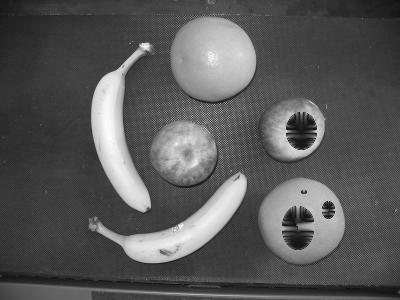
\includegraphics[scale=0.7]{fruitdilatation19.png}
\end{center}

\subsection{Diffusion de la texture}
\begin{center}
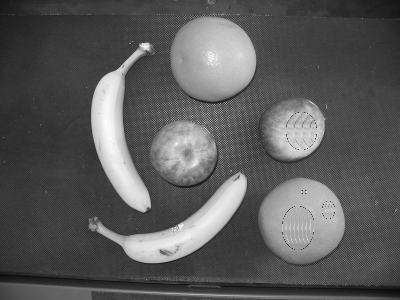
\includegraphics[scale=0.7]{fruitTexture.png}
\end{center}

\newpage
\section{Application des techniques de restauration d'images}
L'orange est détectée manuellement.
\begin{center}
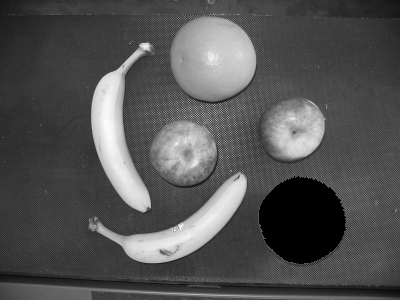
\includegraphics[scale=0.7]{fruit1_boir.png}
\end{center}

\begin{center}
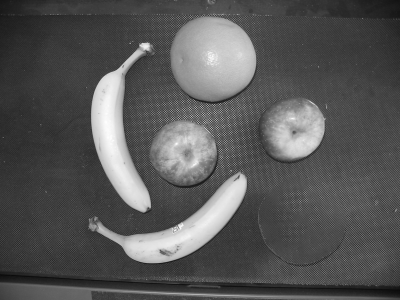
\includegraphics[scale=0.7]{fruit1_photo.png}
\end{center}

\end{document}